\makeatletter
\def\input@path{{../styles/}{../../styles/}{../../../styles/}{../}{../../}{../../../}}
\makeatother
\documentclass{ee102_notes}
% macros.tex - Course meta information
\renewcommand{\course}{EE 102}
\renewcommand{\coursetitle}{Signal Processing and Linear Systems}
\renewcommand{\instructor}{Ayush Pandey}
\renewcommand{\semester}{Fall}
\renewcommand{\year}{2025}
\renewcommand{\shorttitle}{Week 1: Introduction to Signals}
% Use \renewcommand to avoid 'already defined' errors

% The following packages can be found on http:\\www.ctan.org
% \usepackage{graphics} % for pdf, bitmapped graphics files
%\usepackage{epsfig} % for postscript graphics files
%\usepackage{mathptmx} % assumes new font selection scheme installed
%\usepackage{times} % assumes new font selection scheme installed
\usepackage{amsmath} % assumes amsmath package installed
\usepackage{amssymb,mathtools}  % assumes amsmath package installed
\usepackage{xcolor}
\usepackage{pgfplots,subcaption}
\usepackage[hidelinks]{hyperref}
\usepackage{verbatim}
\usepackage{graphicx}
\usepackage{listings}

% -------- listings (Python) ----------
\lstdefinestyle{py}{
  language=Python,
  basicstyle=\ttfamily\small,
  keywordstyle=\color{blue!60!black}\bfseries,
  commentstyle=\color{green!40!black},
  stringstyle=\color{orange!60!black},
  showstringspaces=false,
  columns=fullflexible,
  frame=single,
  framerule=0.3pt,
  numbers=left,
  numberstyle=\tiny,
  xleftmargin=1em,
  tabsize=2,
  breaklines=true,
}
\usepackage[american]{circuitikz}
\usepackage{tikz}
\usepackage{caption}    
\usepackage{lscape}
\usepackage{soul}
\usepackage{tikz}
\usetikzlibrary{calc,angles,quotes,arrows.meta}

\usepackage{hyperref}
\hypersetup{
    colorlinks=true,
    linkcolor=blue,
    filecolor=magenta,      
    urlcolor=blue,
    pdftitle={week1_notes},
    pdfpagemode=FullScreen,
}
%\usepackage{float} 

%\usepackage[demo]{graphicx}
\pgfplotsset{compat=1.18}
% \usepgfplotslibrary{fillbetween}

\newsavebox{\measurebox}

\let\proof\relax\let\endproof\relax


\newcommand{\norm}[1]{\left\lVert#1\right\rVert}
\def\abs#1{\left\lvert#1\right\rvert}
\let\proof\relax
\let\endproof\relax
\usepackage{amsthm}
\usepackage{accents}
\usepackage{relsize}
\newcommand{\ubar}[1]{\underaccent{\bar}{#1}}
\newtheorem{theorem}{Theorem}
\newtheorem{corollary}{Corollary}[theorem]
\newtheorem{lemma}{Lemma}
\newtheorem{proposition}{Proposition}
\newtheorem{statement}{Statement}

\theoremstyle{definition}
\newtheorem{definition}{Definition}
 
\theoremstyle{remark}
\newtheorem*{remark}{Remark}
\theoremstyle{remark}
\newtheorem*{claim}{Claim}
\setlength{\parindent}{0cm}
\newenvironment{nalign}{
    \begin{equation}
    \begin{aligned}
}{
    \end{aligned}
    \end{equation}
    \ignorespacesafterend
}

\renewcommand{\releasedate}{November 19, 2025}
\newcommand{\Eblank}{\rule{3cm}{0.4pt}}
\newcommand{\Rankblank}{\rule{3cm}{0.4pt}}

\begin{document}

\section*{EE 102 Week 12, Lecture 2 (Fall 2025)}
\subsection*{Instructor: \instructor}
\subsection*{Date: \releasedate}
{\color{blue} Note: Week 12 Lecture 1 and Lecture 2 have the mostly the same set of lecture notes. The last section in lecture 2 is the only extra section.}

\section{Announcements}
\begin{itemize}
    \item HW \#10 is due on Mon Nov 17.
    \item HW \#11 will be released Tue Nov 18 and due on Mon Nov 25.
\end{itemize}
\section{Goals}
By the end of this lecture, you should be able to understand the process of sampling a continuous-time signal and how the original signal can be reconstructed from the discrete samples. You will learn to distinguish between the sampling rate, the frequency of the original signal, and the frequencies in the sampled signal. Finally, you will be able to understand that if you keep on increasing the number of samples for a signal, your reconstructed signal will get closer and closer to the original signal. The lower number of samples you take, the more distorted your reconstructed signal will be. But there is a minimum number of samples you must take in order to capture all frequency information of the original signal without distortion. This minimum sampling rate is called the Nyquist rate.
\section{Introduction to Sampling: A Cosine Example}
In this section we connect what you saw in the in-class activity (sampling different
signals at different rates) to the frequency-domain view of sampling and the
Nyquist rate. We will use a single cosine as our starting point:
\[
x(t) = \cos(\omega_0 t),
\]
where $\omega_0$ is the angular frequency in rad/s.

% We will:
% \begin{enumerate}
%     \item Write the sampled signal using an impulse train and the sifting property.
%     \item Derive the sampling period $T_s$, sampling frequency $F_s$, and sampling
%           angular frequency $\omega_s$.
%     \item Carefully derive the Fourier transform of a train of impulses.
%     \item Use that result to derive the spectrum of the sampled signal $X_s(\omega)$.
%     \item See how ``extra'' impulses in $X_s(\omega)$ lead to aliasing if we are not careful.
%     \item Motivate reconstruction by an ideal low-pass filter and arrive at the Nyquist rate.
% \end{enumerate}

The process that we will follow will start by writing the sampled signal in time-domain using impulses. Then, to meet our learning goal of understanding the frequency-domain view of sampling --- that is, we want to find out the minimum number of samples needed to capture all frequency information of the original signal without distortion --- we will derive the Fourier transform of the sampled signal. Using the frequency domain representation of the sampled signal, we will be able to comment on the minimum sampling rate needed and any other extra steps needed to ensure that we can reconstruct the original signal's frequencies without distortion.

\subsection{Sampling in time using an impulse train}

A continuous-time signal $x(t)$ is sampled every $T_s$ seconds. The sampling instants
are
\[
t_n = nT_s, \quad n = 0, \pm 1, \pm 2, \dots
\]
The sampled signal can be written in continuous time as a train of weighted impulses:
\begin{equation}
x_s(t) = \sum_{n=-\infty}^{\infty} x(nT_s)\,\delta(t - nT_s).
\label{eq:sampling_time_domain}
\end{equation}


This expression comes directly from the \textbf{sifting property} of the impulse that we have discussed before:
\[
\int_{-\infty}^{\infty} x(t)\,\delta(t - t_0)\,dt = x(t_0).
\]
Each term $x(nT_s)\,\delta(t - nT_s)$ is zero everywhere except at $t = nT_s$, and
if we integrate $x_s(t)$, only those points contribute. So, the summation above holds.

\begin{popquiz}
Define the sampling period $T_s$, the seconds between samples, on a graph. Find out the sampling frequency $F_s$ (in Hz) and the sampling angular frequency $\omega_s$ (in rad/s) using $T_s$. 
\popqsplit
The sampling period $T_s$ is the time interval between two consecutive samples. See the graph below for reference:
\begin{center}
    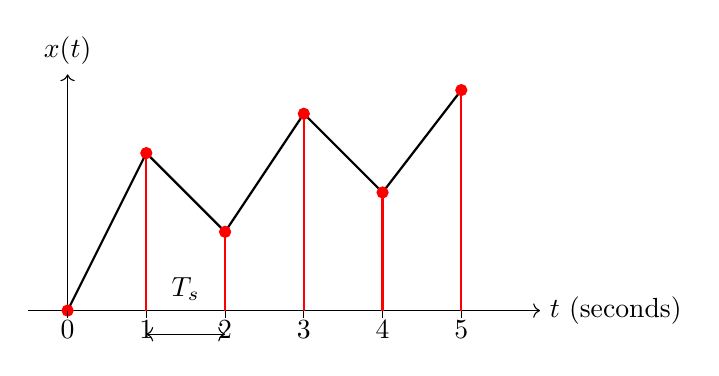
\begin{tikzpicture}
        \draw[->] (-0.5,0) -- (6,0) node[right] {$t$ (seconds)};
        \draw[->] (0,0) -- (0,3) node[above] {$x(t)$};
        % set all y coordinates values as variables
        \def\yzero{0}
        \def\yone{2}
        \def\ytwo{1}
        \def\ythree{2.5}
        \def\yfour{1.5}
        \def\yfive{2.8}
        % draw points and connect them
        \draw[thick] (0,\yzero) -- (1,\yone) -- (2,\ytwo) -- (3,\ythree) -- (4,\yfour) -- (5,\yfive);
        \foreach \x in {0,1,2,3,4,5} {
            % \draw[red,thick] (\x,0) -- (\x,2.8);
            % draw red impulse from \x,0 to \x, (value of y)
            \draw[red,thick] (\x,0) -- (\x,{ifthenelse(\x==0,\yzero,ifthenelse(\x==1,\yone,ifthenelse(\x==2,\ytwo,ifthenelse(\x==3,\ythree,ifthenelse(\x==4,\yfour,\yfive)))))});
            \filldraw[red] (\x,{ifthenelse(\x==0,\yzero,ifthenelse(\x==1,\yone,ifthenelse(\x==2,\ytwo,ifthenelse(\x==3,\ythree,ifthenelse(\x==4,\yfour,\yfive)))))}) circle (2pt);
            % draw sample time ticks
            \draw (\x,0) -- (\x,-0.1);
            % label the ticks 1, 2, 3, ...
            \node[below] at (\x,0) {\x};

        }
        \node[above] at (1.5,0) {$T_s$};
        \draw[<->] (1, -0.3) -- (2, -0.3);
    \end{tikzpicture}
\end{center}
The sampling frequency $F_s$ is the number of samples taken per second, which is the reciprocal of the sampling period:
\[
F_s = \frac{1}{T_s}\quad[\text{samples/second}].
\]
The sampling angular frequency is
\[
\omega_s = 2\pi F_s = \frac{2\pi}{T_s}.
\]
\end{popquiz}

Our goal is to reconstruct the original frequency content of $x(t)$, in this case, the cosine frequency $\omega_0$, from the sampled signal $x_s(t)$. To do this, we will analyze the frequency-domain representation of the sampled signal $x_s(t)$ next.

\subsection*{Fourier transform of the sampled signal}

The signal that we are interested in finding the frequency domain representation of is the sampled signal: $x_s(t)$. Spec ifically, we want to see whether the frequency domain representation of the sampled signal $X_s(\omega)$ contains the original frequency $\omega_0$ of the cosine signal $x(t) = \cos(\omega_0 t)$, and if so, under what conditions (how many sampled do we need to ensure that we get the original frequency $\omega_0$ in $X_s(\omega) $ without any distortion).
We will do this in several steps. 

\subsubsection{Fourier transform of the original cosine}
First, we look at the Fourier transform of the original cosine signal $x(t) = \cos(\omega_0 t)$. Using Euler's relation we can write the cosine as a sum of complex exponentials:
\[
\cos(\omega_0 t) = \frac{1}{2}\left(e^{j\omega_0 t} + e^{-j\omega_0 t}\right).
\]
Now, using the CTFT definition
\[
X(\omega) = \int_{-\infty}^{\infty} x(t)\,e^{-j\omega t}\,dt,
\]
we know the transform of complex exponentials:
\[
\mathcal{F}\{e^{j\omega_0 t}\} = 2\pi\,\delta(\omega - \omega_0),\qquad
\mathcal{F}\{e^{-j\omega_0 t}\} = 2\pi\,\delta(\omega + \omega_0).
\]
Therefore, for $x(t) = \cos(\omega_0 t)$,
\[
X(\omega)
= \frac{1}{2}\bigl[2\pi\,\delta(\omega-\omega_0) + 2\pi\,\delta(\omega+\omega_0)\bigr]
= \pi\bigl[\delta(\omega-\omega_0) + \delta(\omega+\omega_0)\bigr].
\]
So the spectrum of a cosine consists of two impulses, one at $+\omega_0$ and one at $-\omega_0$.

\subsubsection{Fourier transform of a train of impulses}

Now we need the Fourier transform of a periodic impulse train, which we use to model the sampling process. Note that we have the train of impulse signal 
\[
p(t) = \sum_{n=-\infty}^{\infty} \delta(t - nT_s)
\]
multiplied with the original signal $x(t)$ to get the sampled signal $x_s(t)$ (see equation~\eqref{eq:sampling_time_domain}). This is a train of impulses spaced $T_s$ seconds apart. We observe that $p(t)$ is
periodic in time with period $T_s$ since
\[
p(t + T_s) = p(t) \quad \text{for all } t.
\]
\begin{popquiz}
    Plot the train of impulse signal $p(t)$. Visually and mathematically verify that $p(t)$ is periodic with period $T_s$.
    \popqsplit
    The plot of the train of impulse signal $p(t)$ is shown below:
    \begin{center}
    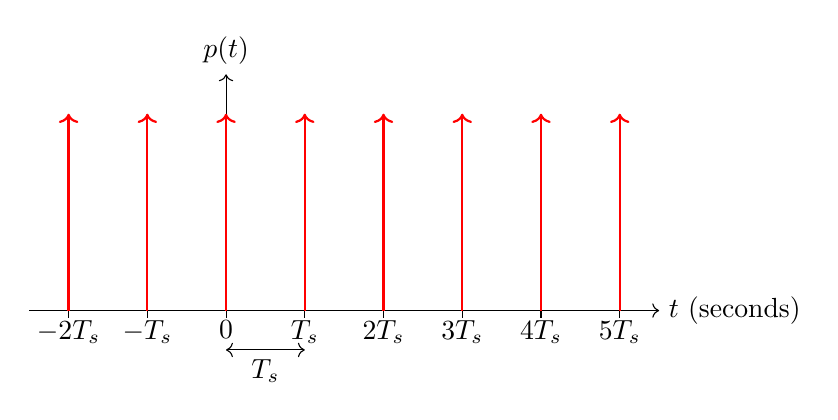
\begin{tikzpicture}
        % axes
        \draw[->] (-2.5,0) -- (5.5,0) node[right] {$t$ (seconds)};
        \draw[->] (0,0) -- (0,3) node[above] {$p(t)$};

        % draw red impulses at t = -2Ts, -Ts, 0, Ts, 2Ts, 3Ts, 4Ts, 5Ts
        \foreach \x in {-2,-1,0,1,2,3,4,5} {
            \draw[red,thick,->] (\x,0) -- (\x,2.5);
            % tick at the time axis
            \draw (\x,0) -- (\x,-0.1);
        }

        % labels for the ticks: -2Ts, -Ts, 0, Ts, 2Ts, 3Ts, 4Ts, 5Ts
        \node[below] at (-2,0) {$-2T_s$};
        \node[below] at (-1,0) {$-T_s$};
        \node[below] at ( 0,0) {$0$};
        \node[below] at ( 1,0) {$T_s$};
        \node[below] at ( 2,0) {$2T_s$};
        \node[below] at ( 3,0) {$3T_s$};
        \node[below] at ( 4,0) {$4T_s$};
        \node[below] at ( 5,0) {$5T_s$};

        % double arrow from 0 to Ts
        \draw[<->] (0, -0.5) -- (1, -0.5);
        \node[below] at (0.5,-0.5) {$T_s$};
    \end{tikzpicture}
    \end{center}

    To verify that $p(t)$ is periodic with period $T_s$, we check that $p(t + T_s) = p(t)$ for all $t$:
    \[
    p(t + T_s) = \sum_{n=-\infty}^{\infty} \delta(t + T_s - nT_s) = \sum_{n=-\infty}^{\infty} \delta(t - (n-1)T_s).
    \]
    By changing the index of summation from $n$ to $m = n - 1$, we have
    \[
    p(t + T_s) = \sum_{m=-\infty}^{\infty} \delta(t - mT_s) = p(t).
    \]
\end{popquiz}
Because $p(t)$ is periodic, we can represent it as a sum of complex exponentials using its Fourier series. This will help us compute its Fourier transform more easily. We have 
\[
p(t) = \sum_{k=-\infty}^{\infty} c_k\,e^{jk\omega_s t},
\quad \text{with} \quad
\omega_s = \frac{2\pi}{T_s},
\]
and the Fourier series coefficients are
\[
c_k = \frac{1}{T_s} \int_{0}^{T_s} p(t)\,e^{-jk\omega_s t}\,dt,
\]
Recall from \href{https://github.com/ee-ucmerced/ee102-signals-systems/blob/main/homework/week6/hw6.pdf}{Homework \#6 Problem 1} that the Fourier series coefficients for a periodic impulse train is
\[
c_k = \frac{1}{T_s} \quad \text{for all } k, \quad \text{so \quad }
p(t) = \frac{1}{T_s} \sum_{k=-\infty}^{\infty} e^{jk\omega_s t}.
\]

Now we take the Fourier transform of $p(t)$. Using linearity:
\[
P(\omega) = \mathcal{F}\{p(t)\}
= \frac{1}{T_s} \sum_{k=-\infty}^{\infty}
   \mathcal{F}\{e^{jk\omega_s t}\}.
\]
From \href{https://github.com/ee-ucmerced/ee102-signals-systems/blob/main/lecture_notes/week11_frequency_domain_2/week11_lecture1.pdf}{Pop quiz 3.1 in week 11 lecture 1}, we know that the Fourier transform of a complex exponential is
\[
\mathcal{F}\{e^{j\omega_0 t}\} = 2\pi\,\delta(\omega - \omega_0).
\]
Here, $\omega_0 = k\omega_s$, so
\[
\mathcal{F}\{e^{jk\omega_s t}\} = 2\pi\,\delta(\omega - k\omega_s).
\]
Therefore
\[
P(\omega)
= \frac{2\pi}{T_s} \sum_{k=-\infty}^{\infty} \delta(\omega - k\omega_s).
\]

So, finally, we can write that the Fourier transform of a periodic impulse train with period $T_s$ is a train
of impulses in the frequency domain (how convenient!)! The impulses in the frequency domain are spaced by $\omega_s = \dfrac{2\pi}{T_s}$ --- the sampling frequency. So, we have the pair:
\[
p(t) = \sum_{n=-\infty}^{\infty} \delta(t - nT_s)
\quad\Longleftrightarrow\quad
P(\omega) = \frac{2\pi}{T_s} \sum_{k=-\infty}^{\infty} \delta(\omega - k\omega_s).
\]

Now are ready to compute the Fourier transform of the sampled signal $x_s(t)$.
\subsection*{Fourier transform of the sampled signal: multiplication of $p(t)$ and $x(t)$}

Sampling a signal $x(t)$, as in equation~\eqref{eq:sampling_time_domain}, can be viewed as multiplying the original signal $x(t)$ by the impulse train $p(t)$. How? See below:
\[
x_s(t) = x(t)\,p(t)
= x(t)\sum_{n=-\infty}^{\infty} \delta(t - nT_s)
= \sum_{n=-\infty}^{\infty} x(t)\,\delta(t - nT_s).
\]

Using the sifting property inside the sum:
\[
x_s(t) = \sum_{n=-\infty}^{\infty} x(nT_s)\,\delta(t - nT_s),
\]
which matches our original expression in equation~\eqref{eq:sampling_time_domain}. Now, our goal is to compute the frequency domain representation of the sampled signal $x_s(t)$ by computing its Fourier transform. 

In the frequency domain, multiplication in time corresponds to \emph{convolution} in frequency. We have not seen this explicitly but you may get the intuition for why this holds true from the duality between time and frequency domains. Specifically, recall that when we convolve two signals in time domain, that is, if we have $y(t) = x(t) * h(t)$, then in the frequency domain, we have $Y(\omega) = X(\omega)H(\omega)$ --- multiplication in frequency! So, by duality, it holds true that multiplication in time corresponds to convolution in frequency. You may find a proof of this property in Chapter 4 of Oppenheim and Willsky's Signals and Systems textbook (2nd Edition). We use this property here to compute the Fourier transform of the sampled signal $x_s(t)$. We have 
\[
X_s(\omega) = \frac{1}{2\pi} \bigl[X(\omega) * P(\omega)\bigr],
\]
where $X(\omega)$ and $P(\omega)$ are the Fourier transforms of $x(t)$ and $p(t)$ respectively (the $1/2\pi$ factor comes from the multiplication property of the Fourier transform) Now, substituting $P(\omega)$, we have
\[
X_s(\omega)
= \frac{1}{2\pi} X(\omega) * \left( \frac{2\pi}{T_s} \sum_{k=-\infty}^{\infty}
\delta(\omega - k\omega_s) \right)
= \frac{1}{T_s} \left[ X(\omega) * \sum_{k=-\infty}^{\infty} \delta(\omega - k\omega_s) \right].
\]
Again, recall a property of Fourier transforms that the convolution with a shifted delta shifts the function. So, 
\[
X(\omega) * \delta(\omega - a) = X(\omega - a).
\]
\[
X_s(\omega)
= \frac{1}{T_s} \sum_{k=-\infty}^{\infty} X(\omega - k\omega_s).
\]

Therefore, we get that the frequency domain representation of the sampled signal $X_s(\omega)$ is
a scaled sum of shifted copies of the original spectrum $X(\omega)$ (not ideal!), shifted
by multiples of $\omega_s$.

For our cosine example, we have already computed $X(\omega)$:
\[
X(\omega) = \pi\bigl[\delta(\omega-\omega_0) + \delta(\omega+\omega_0)\bigr]
\]
which gives us 
\[
X_s(\omega)
= \frac{1}{T_s} \sum_{k=-\infty}^{\infty} X(\omega - k\omega_s)
= \frac{1}{T_s} \sum_{k=-\infty}^{\infty}
\pi\bigl[\delta(\omega - k\omega_s - \omega_0)
       + \delta(\omega - k\omega_s + \omega_0)\bigr].
\]

So $X_s(\omega)$ has impulses at
\[
\omega = \pm\omega_0 + k\omega_s, \qquad k \in \mathbb{Z}.
\]
The original two impulses at $\pm\omega_0$ are now repeated (copied) at integer multiples
of the sampling frequency $\omega_s$!!! This is not great, because now the sampled
signal contains many more frequency components than the original signal (these are the distortions that you hear when you don't sample correctly!). How can we remove these additional impulses and recover the original cosine frequency $\omega_0$? Low pass filtering! We will discuss this in more detail next time. 

\subsection*{Filtering to remove distortions}

The original continuous-time cosine only had two impulses 
at $\omega = \pm\omega_0$. After sampling, $X_s(\omega)$ contains infinitely
many impulses, at
\[
\omega = \pm\omega_0, \quad
\pm\omega_0 \pm \omega_s, \quad
\pm\omega_0 \pm 2\omega_s, \quad \dots
\]

If $\omega_s$ is large enough, these copies are separated in frequency and do not overlap.
But if $\omega_s$ is too small, the shifted impulses can collide or cross into each other.
In other words, impulses from different ``copies'' of $X(\omega)$ may end up in the same
frequency location. This leads to distortion in the reconstructed signal called aliasing.

\textbf{What is aliasing?} When the sampling frequency is too low,
different frequency components in the original signal produce overlapping or indistinguishable
contributions in the sampled spectrum. In the reconstructed signal, these contributions
appear as \emph{fake} or \emph{misplaced} frequencies. This phenomenon is called \textbf{aliasing}:
different original frequencies become indistinguishable after sampling.

For a single cosine, aliasing means that a high-frequency cosine can ``look like'' a lower-frequency cosine once sampled, because their impulses line up after shifts
by $\omega_s$.


As we said above, to reconstruct the original continuous-time signal $x(t)$ from its samples, we may design a low-pass filter to remove the extra copies in $X_s(\omega)$. This will work only if the copies do not overlap with the original spectrum. An ideal low-pass filter has a cutoff frequency $\omega_c$ that passes only the frequency band containing the original $X(\omega)$ (from $-\omega_c$ to $+\omega_c$) and removes all higher frequencies will work well.

For a single cosine at $\omega_0$, we can choose the cutoff frequency $\omega_c$ such that
\[
\omega_0 < \omega_c < \omega_s - \omega_0.
\]
This is possible \emph{only if} the original impulse at $+\omega_0$ is strictly
separated from the nearest shifted impulse at $\omega_s - \omega_0$. That gives the
inequality
\[
\omega_0 < \omega_s - \omega_0
\quad \Longleftrightarrow \quad
\omega_s > 2\omega_0.
\]

Under this condition, an ideal low-pass filter with passband
$|\omega| < \omega_c$ will keep the original impulses at $\pm\omega_0$ and completely remove all impulses from the shifted copies.
In the time domain, this low-pass filter reconstructs the original continuous-time cosine
$x(t) = \cos(\omega_0 t)$ from the samples (our overall goal!). The condition that we just obtained is called the \textbf{Nyquist sampling condition}.

We have shown that to avoid overlap between the original impulses at $\pm\omega_0$
and the nearest replicated impulses (at $\pm\omega_0 \pm \omega_s$), we must have
\[
\omega_s > 2\omega_0.
\]

We can obtain an equivalent relation in Hz. Recall $\omega_s = \dfrac{2\pi}{T_s}$ and $\omega_0 = 2\pi f_0$ where $f_0$ is the
ordinary frequency in Hz. In terms of the sampling frequency $F_s = 1/T_s$:
\[
\omega_s > 2\omega_0
\quad\Longleftrightarrow\quad
2\pi F_s > 2(2\pi f_0)
\quad\Longleftrightarrow\quad
F_s > 2f_0.
\]

So, the Nyquist rate for a single cosine:
\[
F_s > 2f_0, \qquad f_0 = \frac{\omega_0}{2\pi}.
\]
If we sample \emph{above} this Nyquist rate, we can in principle use an ideal
low-pass filter to remove the extra copies in $X_s(\omega)$ and reconstruct the
original cosine exactly from its samples. This is the key result of this week's theoretical topics.

\section{Nyquist Sampling Theorem}
We end with the formal statement of the Nyquist Sampling Theorem for general bandlimited signals (not just a single cosine).
\begin{theorem}[Nyquist Sampling Theorem]
If a continuous-time signal $x(t)$ contains no frequencies higher than
$B$ Hz, that is, if its Fourier transform $X(\omega)$ is zero for
$|\omega| > 2\pi B$, then $x(t)$ is completely determined by its samples
taken at a sampling frequency $F_s$ greater than $2B$ Hz. In this case,
$x(t)$ can be reconstructed from its samples using an ideal low-pass filter. 
\end{theorem}

\section{Recommended Reading}
Run \href{https://github.com/ee-ucmerced/ee102-signals-systems/blob/main/lecture_notes/week12_sampling/VM_aliasing.ipynb}{\texttt{VM\_aliasing.ipynb}} notebook that is available on course GitHub. Try to achieve the following using the code:
\begin{itemize}
    \item Visualize aliasing with $x(t) = \sin(2\pi f_0 t)$ for different values of $f_0$ and different sampling frequencies $F_s$.
    \item Observe how increasing the number of samples improves the reconstruction of the original signal for the sine wave.
    \item Apply the sampling theorem to adequately sample and reconstruct your recorded voice from Homework \#10.
\end{itemize}
\end{document}